%\input{Preambulum}

\begin{figure}[t!]
\centering

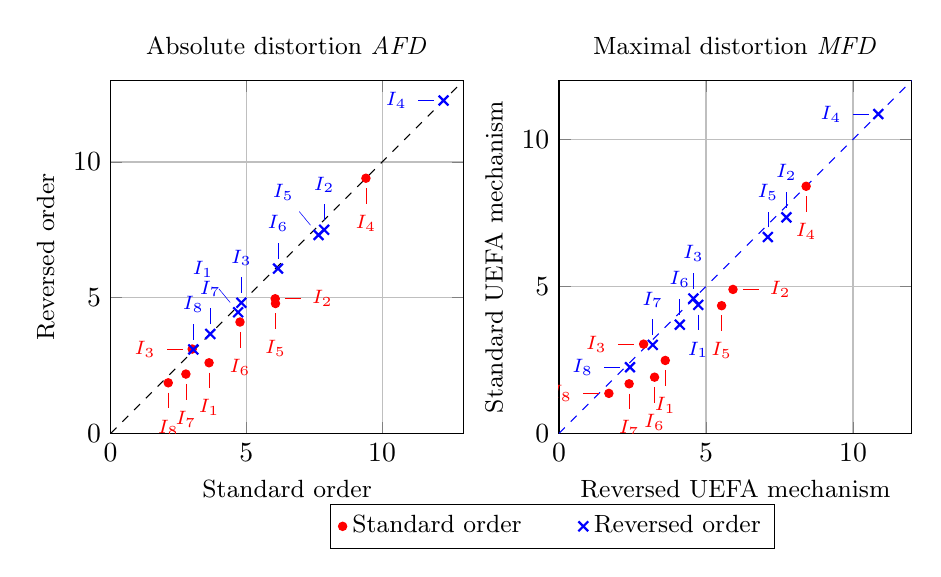
\begin{tikzpicture}
\begin{axis}[
name = axis1,
title = {Absolute distortion $\mathit{AFD}$},
title style = {font=\small},
xlabel = Standard order,
x label style = {font=\small},
ylabel = Reversed order,
y label style = {font=\small},
width = 0.5\textwidth,
height = 0.5\textwidth,
nodes near coords,
xmajorgrids = true,
ymajorgrids = true,
xmin = 0,
xmax = 13,
ymin = 0,
ymax = 13,
]
% Drop mechanism
\addplot [scatter,red,only marks,mark size=1.5pt,point meta=explicit symbolic] coordinates {
%\addplot [scatter,red,only marks,mark size=1.5pt,point meta=explicit symbolic,nodes near coords style = {text=red, anchor=south east}] coordinates {
(3.62579669058374,2.60266248942994)
(6.06312825736648,4.96180950736648)
(3.00423537342155,3.10807620675489)
(9.4048946588799,9.40205721207138)
(6.07375613010738,4.78552130383974)
(4.76576911249559,4.10367422122957)
(2.77228684771103,2.18681711376466)
(2.1222286748029,1.86451868452316)
};
% Zero line
\draw [black,dashed] (rel axis cs:0,0) -- (rel axis cs:1,1);
% Labels
\node[pin={[pin distance=0.2cm, ultra thick, pin edge={red}] 270:{\textcolor{red}{\scriptsize{$I_1$}}}}] at (3.62579669058374,2.60266248942994) {};
\node[pin={[pin distance=0.2cm, ultra thick, pin edge={red}] 360:{\textcolor{red}{\scriptsize{$I_2$}}}}] at (6.06312825736648,4.96180950736648) {};
\node[pin={[pin distance=0.2cm, ultra thick, pin edge={red}] 180:{\textcolor{red}{\scriptsize{$I_3$}}}}] at (3.00899370675489,3.09640912342156) {};
\node[pin={[pin distance=0.2cm, ultra thick, pin edge={red}] 270:{\textcolor{red}{\scriptsize{$I_4$}}}}] at (9.4048946588799,9.40205721207138) {};
\node[pin={[pin distance=0.2cm, ultra thick, pin edge={red}] 270:{\textcolor{red}{\scriptsize{$I_5$}}}}] at (6.07375613010738,4.78552130383974) {};
\node[pin={[pin distance=0.2cm, ultra thick, pin edge={red}] 270:{\textcolor{red}{\scriptsize{$I_6$}}}}] at (4.76576911249559,4.10367422122957) {};
\node[pin={[pin distance=0.2cm, ultra thick, pin edge={red}] 270:{\textcolor{red}{\scriptsize{$I_7$}}}}] at (2.77228684771103,2.18681711376466) {};
\node[pin={[pin distance=0.2cm, ultra thick, pin edge={red}] 270:{\textcolor{red}{\scriptsize{$I_8$}}}}] at (2.1222286748029,1.86451868452316) {};
% Skip mechanism
\addplot [scatter,blue,only marks,mark=x,mark size=2.5pt,thick,point meta=explicit symbolic] coordinates {
(4.69816248942994,4.46424248942994)
(7.86677617403314,7.50255659069981)
(4.81761079008822,4.81402802326587)
(12.265759339731,12.2658078503693)
(7.65961789958443,7.31111490246786)
(6.16646911249559,6.07336145292112)
(3.67082378043133,3.66492794709799)
(3.04516555783561,3.09439533210929)
};
% Labels
\node[pin={[pin distance=0.2cm, ultra thick, pin edge={blue}] 120:{\textcolor{blue}{\scriptsize{$I_1$}}}}] at (4.69816248942994,4.46424248942994) {};
\node[pin={[pin distance=0.2cm, ultra thick, pin edge={blue}] 90:{\textcolor{blue}{\scriptsize{$I_2$}}}}] at (7.86677617403314,7.50255659069981) {};
\node[pin={[pin distance=0.2cm, ultra thick, pin edge={blue}] 90:{\textcolor{blue}{\scriptsize{$I_3$}}}}] at (4.81761079008822,4.81402802326587) {};
\node[pin={[pin distance=0.2cm, ultra thick, pin edge={blue}] 180:{\textcolor{blue}{\scriptsize{$I_4$}}}}] at (12.265759339731,12.2658078503693) {};
\node[pin={[pin distance=0.2cm, ultra thick, pin edge={blue}] 120:{\textcolor{blue}{\scriptsize{$I_5$}}}}] at (7.65961789958443,7.31111490246786) {};
\node[pin={[pin distance=0.2cm, ultra thick, pin edge={blue}] 90:{\textcolor{blue}{\scriptsize{$I_6$}}}}] at (6.16646911249559,6.07336145292112) {};
\node[pin={[pin distance=0.2cm, ultra thick, pin edge={blue}] 90:{\textcolor{blue}{\scriptsize{$I_7$}}}}] at (3.67082378043133,3.66492794709799) {};
\node[pin={[pin distance=0.2cm, ultra thick, pin edge={blue}] 90:{\textcolor{blue}{\scriptsize{$I_8$}}}}] at (3.04516555783561,3.09439533210929) {};
\end{axis}

\begin{axis}[
at = {(axis1.south east)},
xshift = 0.1\textwidth,
title = {Maximal distortion $\mathit{MFD}$},
title style = {font=\small},
xlabel = Reversed UEFA mechanism,
x label style = {font=\small},
ylabel = Standard UEFA mechanism,
y label style = {font=\small},
width = 0.5\textwidth,
height = 0.5\textwidth,
nodes near coords,
xmajorgrids = true,
ymajorgrids = true,
xmin = 0,
xmax = 12,
ymin = 0,
ymax = 12,
legend style = {font=\small,at={(-0.65,-0.2)},anchor=north west,legend columns=3},
legend entries = {Standard order$\qquad$,Reversed order}
]
% Drop mechanism
\addplot [scatter,red,only marks,mark size=1.5pt,point meta=explicit symbolic] coordinates {
(3.61513049551676,2.48108549551675)
(5.91848361325967,4.89715361325967)
(2.87850603113648,3.03629703113648)
(8.40618744836776,8.40517144836775)
(5.53118871888203,4.34370771888203)
(3.25062201104973,1.91257101104972)
(2.38603470150833,1.68764170150834)
(1.69718396954315,1.36173696954315)
};
% Zero line
\draw [blue,dashed] (rel axis cs:0,0) -- (rel axis cs:1,1);
% Labels
\node[pin={[pin distance=0.2cm, ultra thick, pin edge={red}] 270:{\textcolor{red}{\scriptsize{$I_1$}}}}] at (3.61513049551676,2.48108549551675) {};
\node[pin={[pin distance=0.2cm, ultra thick, pin edge={red}] 360:{\textcolor{red}{\scriptsize{$I_2$}}}}] at (5.91848361325967,4.89715361325967) {};
\node[pin={[pin distance=0.2cm, ultra thick, pin edge={red}] 180:{\textcolor{red}{\scriptsize{$I_3$}}}}] at (2.87850603113648,3.03629703113648) {};
\node[pin={[pin distance=0.2cm, ultra thick, pin edge={red}] 270:{\textcolor{red}{\scriptsize{$I_4$}}}}] at (8.40618744836776,8.40517144836775) {};
\node[pin={[pin distance=0.2cm, ultra thick, pin edge={red}] 270:{\textcolor{red}{\scriptsize{$I_5$}}}}] at (5.53118871888203,4.34370771888203) {};
\node[pin={[pin distance=0.2cm, ultra thick, pin edge={red}] 270:{\textcolor{red}{\scriptsize{$I_6$}}}}] at (3.25062201104973,1.91257101104972) {};
\node[pin={[pin distance=0.2cm, ultra thick, pin edge={red}] 270:{\textcolor{red}{\scriptsize{$I_7$}}}}] at (2.38603470150833,1.68764170150834) {};
\node[pin={[pin distance=0.2cm, ultra thick, pin edge={red}] 180:{\textcolor{red}{\scriptsize{$I_8$}}}}] at (1.69718396954315,1.36173696954315) {};
% Skip mechanism
\addplot [scatter,blue,only marks,mark=x,mark size=2.5pt,thick,point meta=explicit symbolic] coordinates {
(4.73620549551675,4.37280249551675)
(7.73453161325967,7.34826061325967)
(4.57178503113648,4.58633003113648)
(10.8605964483678,10.8605784483678)
(7.10442771888203,6.67784971888203)
(4.10838101104972,3.69726501104972)
(3.18875970150833,3.01230370150833)
(2.41598696954314,2.25215396954315)
};
% Labels
\node[pin={[pin distance=0.2cm, ultra thick, pin edge={blue}] 270:{\textcolor{blue}{\scriptsize{$I_1$}}}}] at (4.73620549551675,4.37280249551675) {};
\node[pin={[pin distance=0.2cm, ultra thick, pin edge={blue}] 90:{\textcolor{blue}{\scriptsize{$I_2$}}}}] at (7.73453161325967,7.34826061325967) {};
\node[pin={[pin distance=0.2cm, ultra thick, pin edge={blue}] 90:{\textcolor{blue}{\scriptsize{$I_3$}}}}] at (4.57178503113648,4.58633003113648) {};
\node[pin={[pin distance=0.2cm, ultra thick, pin edge={blue}] 180:{\textcolor{blue}{\scriptsize{$I_4$}}}}] at (10.8605964483678,10.8605784483678) {};
\node[pin={[pin distance=0.2cm, ultra thick, pin edge={blue}] 90:{\textcolor{blue}{\scriptsize{$I_5$}}}}] at (7.10442771888203,6.67784971888203) {};
\node[pin={[pin distance=0.2cm, ultra thick, pin edge={blue}] 90:{\textcolor{blue}{\scriptsize{$I_6$}}}}] at (4.10838101104972,3.69726501104972) {};
\node[pin={[pin distance=0.2cm, ultra thick, pin edge={blue}] 90:{\textcolor{blue}{\scriptsize{$I_7$}}}}] at (3.18875970150833,3.01230370150833) {};
\node[pin={[pin distance=0.2cm, ultra thick, pin edge={blue}] 180:{\textcolor{blue}{\scriptsize{$I_8$}}}}] at (2.41598696954314,2.25215396954315) {};
\end{axis}
\end{tikzpicture}

\caption{Fairness distortions of the UEFA mechanisms for the graphs in Figure~\ref{Fig7}}
\label{Fig10}

\end{figure}

%\end{document}